\documentclass[11pt, letterpaper]{article}

% Mandatory Packages
\usepackage{amsmath}
\usepackage{amssymb}
\usepackage{amsthm}
\usepackage{geometry}
\usepackage{tikz}
\usetikzlibrary{arrows.meta, positioning, shapes.geometric, intersections}
\usepackage{mathrsfs}
\usepackage{mathtools}
\usepackage{enumitem}
\usepackage{hyperref}

% Geometry Settings
\geometry{
    top=1in,
    bottom=1in,
    left=1in,
    right=1in
}

% Theorem Environments
\newtheorem{theorem}{Theorem}[section]
\newtheorem{lemma}[theorem]{Lemma}
\newtheorem{proposition}[theorem]{Proposition}
\newtheorem{corollary}[theorem]{Corollary}
\theoremstyle{definition}
\newtheorem{definition}{Definition}[section]
\newtheorem{axiom}{Axiom}[section]
\theoremstyle{remark}
\newtheorem{remark}{Remark}[section]

% Custom Commands for Math Mode Rigor
\newcommand{\R}{\mathbb{R}}
\newcommand{\N}{\mathbb{N}}
\newcommand{\Z}{\mathbb{Z}}
\newcommand{\Q}{\mathbb{Q}}
\newcommand{\F}{\mathscr{F}}
\newcommand{\Prob}{\mathbb{P}}
\newcommand{\E}{\mathbb{E}}
\newcommand{\comp}[1]{\overline{#1}}
\DeclarePairedDelimiter{\abs}{\lvert}{\rvert}

% Title, Author, Date
\title{\textbf{Homework 2: Set Theory, Combinatorics, and Axiomatic Probability}}
\author{
    \textbf{Tashfeen Hatim Said Omran} \\ 
    UCF ID: 5862894 \\ 
    Class: STA4321
}
\date{September 2026}

\begin{document}

\maketitle
\tableofcontents
\newpage

% ======================================================================= %
\section{Part 1: Comprehensive Introduction, Context, and Prerequisites}
% ======================================================================= %

\subsection{Historical Context and Motivation}
Historically, probability was formalized in the 17th century by mathematicians such as Blaise Pascal and Pierre de Fermat to solve problems related to games of chance. However, this classical approach---which relied heavily on counting equally likely outcomes---was ill-equipped to handle continuous variables, infinite sequences of events, or rigorous proofs of convergence. The foundational crisis of probability was resolved in 1933 when Andrey Kolmogorov published \textit{Foundations of the Theory of Probability}. Kolmogorov revolutionized the field by anchoring probability strictly to measure theory and set theory, treating random events as sets within a universal sample space and defining probability as a normalized measure. This axiomatic framework is what allows us to safely transition from basic combinatorics to advanced Stochastic Calculus and Machine Learning models today.

\subsection{Core Concepts, Axioms, and Logical Foundations}
To operate with theoretical rigor, we must define the mathematical spaces governing probability.

\begin{definition}[Sample Space]
The sample space, denoted $\Omega$ (or $S$), is the set of all possible outcomes of a random experiment.
\end{definition}

\begin{definition}[$\sigma$-algebra]
A collection of subsets of $\Omega$, denoted $\mathscr{F}$, is a $\sigma$-algebra if it satisfies three properties:
1. $\Omega \in \mathscr{F}$.
2. If $A \in \mathscr{F}$, then its complement $\comp{A} \in \mathscr{F}$.
3. If $A_{1}, A_{2}, \dots \in \mathscr{F}$, then $\bigcup_{i=1}^{\infty} A_{i} \in \mathscr{F}$.
\end{definition}

\begin{axiom}[Kolmogorov's Axioms of Probability]
Let $\Omega$ be a sample space and $\mathscr{F}$ be a $\sigma$-algebra over $\Omega$. A probability measure is a function $\mathbb{P}: \mathscr{F} \to \mathbb{R}$ satisfying:
\begin{enumerate}
    \item \textbf{Non-negativity:} For any event $A \in \mathscr{F}$, $\mathbb{P}(A) \ge 0$.
    \item \textbf{Normalization:} $\mathbb{P}(\Omega) = 1$.
    \item \textbf{Countable Additivity:} If $A_{1}, A_{2}, \dots$ are mutually exclusive events (i.e., $A_{i} \cap A_{j} = \emptyset$ for $i \ne j$), then $\mathbb{P}\left(\bigcup_{i=1}^{\infty} A_{i}\right) = \sum_{i=1}^{\infty} \mathbb{P}(A_{i})$.
\end{enumerate}
\end{axiom}

\subsection{Key Theorems and Combinatorial Formulas}
\begin{itemize}
    \item \textbf{Distributive Laws of Set Theory:} $A \cap (B \cup C) = (A \cap B) \cup (A \cap C)$.
    \item \textbf{Law of Total Probability (Partitioning):} For any set $A$ and a set $B$, $A = (A \cap B) \cup (A \cap \comp{B})$.
    \item \textbf{Multiplication Principle:} If a process consists of $k$ independent steps, and the $i$-th step can be done in $n_{i}$ ways, the total number of outcomes is $\prod_{i=1}^{k} n_{i}$.
    \item \textbf{Permutations:} The number of ways to choose $k$ distinct ordered items from $n$ items is $P(n, k) = \frac{n!}{(n-k)!}$.
    \item \textbf{Combinations:} The number of ways to choose $k$ items from $n$ distinct items where order does not matter is $\binom{n}{k} = \frac{n!}{k!(n-k)!}$.
    \item \textbf{Multinomial Coefficient:} The number of ways to partition $n$ distinct objects into $k$ distinct groups of sizes $n_{1}, n_{2}, \dots, n_{k}$ where $\sum n_{i} = n$ is $\binom{n}{n_{1}, n_{2}, \dots, n_{k}} = \frac{n!}{n_{1}!n_{2}!\dots n_{k}!}$.
\end{itemize}

\subsection{Prerequisites}
Mastery of this chapter requires foundational set operations (unions, intersections, complements, and subsets), a firm grasp of algebraic manipulation, basic counting intuition (stars and bars, distinct vs. identical items), and the ability to formulate Direct Proofs using element-chasing techniques.

\newpage
% ======================================================================= %
\section{Part 2: Detailed Homework Solutions (Rigorous Proofs)}
% ======================================================================= %

\subsection*{Problem 2.4 / 2.5}
\textbf{Prompt:} Use the identities $A = A \cap S$ and $S = B \cup \comp{B}$ and a distributive law to prove that:
\textbf{a)} $A = (A \cap B) \cup (A \cap \comp{B})$.
\textbf{b)} If $B \subset A$ then $A = B \cup (A \cap \comp{B})$.
\textbf{c)} Show that $(A \cap B)$ and $(A \cap \comp{B})$ are mutually exclusive and therefore that $A$ is the union of two mutually exclusive sets.
\textbf{d)} Show that $B$ and $(A \cap \comp{B})$ are mutually exclusive and if $B \subset A$, $A$ is the union of two mutually exclusive sets, $B$ and $(A \cap \comp{B})$.

\begin{proof}[Solution to 2.5 (a)]
By definition of the universal set (sample space) $S$, every set $A$ satisfies $A \subset S$, hence:
\[ A = A \cap S \]
We are given the identity $S = B \cup \comp{B}$, which is the Law of Excluded Middle applied to sets. Substituting this into our first equation yields:
\[ A = A \cap (B \cup \comp{B}) \]
Applying the set-theoretic Distributive Law of Intersection over Union, we obtain:
\[ A = (A \cap B) \cup (A \cap \comp{B}) \]
\end{proof}

\begin{proof}[Solution to 2.5 (b)]
Assume $B \subset A$. By definition of a subset, every element of $B$ is an element of $A$, which implies that the intersection of $A$ and $B$ is exactly $B$. Formally:
\[ A \cap B = B \]
From part (a), we established that $A = (A \cap B) \cup (A \cap \comp{B})$. Substituting $B$ for $(A \cap B)$ in this established identity gives:
\[ A = B \cup (A \cap \comp{B}) \]
\end{proof}

\begin{proof}[Solution to 2.5 (c)]
Two sets $X$ and $Y$ are mutually exclusive if their intersection is the empty set, $X \cap Y = \emptyset$. We evaluate the intersection of $(A \cap B)$ and $(A \cap \comp{B})$:
\begin{align*}
(A \cap B) \cap (A \cap \comp{B}) &= A \cap A \cap B \cap \comp{B} \quad &&\text{(Associative and Commutative Laws)} \\
&= A \cap (B \cap \comp{B}) \quad &&\text{(Idempotent Law: } A \cap A = A) \\
&= A \cap \emptyset \quad &&\text{(Contradiction Law: } B \cap \comp{B} = \emptyset) \\
&= \emptyset \quad &&\text{(Domination Law)}
\end{align*}
Since their intersection is $\emptyset$, $(A \cap B)$ and $(A \cap \comp{B})$ are mutually exclusive. Hence, the identity $A = (A \cap B) \cup (A \cap \comp{B})$ expresses $A$ as the union of two mutually exclusive sets.
\end{proof}

\begin{proof}[Solution to 2.5 (d)]
We evaluate the intersection of $B$ and $(A \cap \comp{B})$:
\begin{align*}
B \cap (A \cap \comp{B}) &= (B \cap \comp{B}) \cap A \quad &&\text{(Commutativity and Associativity)} \\
&= \emptyset \cap A \quad &&\text{(Contradiction Law)} \\
&= \emptyset \quad &&\text{(Domination Law)}
\end{align*}
Thus, $B$ and $(A \cap \comp{B})$ are mutually exclusive. If $B \subset A$, we proved in part (b) that $A = B \cup (A \cap \comp{B})$. Since the two sets forming this union are mutually exclusive, $A$ is the union of two mutually exclusive sets.
\end{proof}

% ----------------------------------------------------------------------- %
\subsection*{Problem 2.8}
\textbf{Prompt:} Two dice are tossed. Let $S$ denote the set of all possible pairs $(x,y)$.
\textbf{a)} Define subsets: $A$: number on second die is even. $B$: sum of the two numbers is even. $C$: at least one number is odd.
\textbf{b)} List the points in $A$, $\comp{C}$, $A \cap B$, $A \cap \comp{B}$, $\comp{A} \cup B$, and $\comp{A} \cap C$.

\textbf{Solution:}
Let the sample space be $S = \{(x,y) \mid x \in \{1,2,3,4,5,6\}, y \in \{1,2,3,4,5,6\}\}$. The cardinality of $S$ is $|S| = 36$.
\textbf{Part a: Set Definitions}
\begin{itemize}
    \item $A = \{(x,y) \in S \mid y \in \{2,4,6\}\}$
    \item $B = \{(x,y) \in S \mid (x+y) \bmod 2 = 0\} = \{(x,y) \in S \mid (x,y \text{ both even}) \lor (x,y \text{ both odd})\}$
    \item $C = \{(x,y) \in S \mid (x \bmod 2 \ne 0) \lor (y \bmod 2 \ne 0)\}$
\end{itemize}

\textbf{Part b: Point Listings}
\begin{enumerate}[label=\arabic*.]
    \item \textbf{Points in $A$}: (18 points)
    \[ A = \left\{ \begin{array}{l} (1,2), (2,2), (3,2), (4,2), (5,2), (6,2), \\ (1,4), (2,4), (3,4), (4,4), (5,4), (6,4), \\ (1,6), (2,6), (3,6), (4,6), (5,6), (6,6) \end{array} \right\} \]
    
    \item \textbf{Points in $\comp{C}$}: The complement of ``at least one odd'' is ``both are even''. (9 points)
    \[ \comp{C} = \{(2,2), (2,4), (2,6), (4,2), (4,4), (4,6), (6,2), (6,4), (6,6)\} \]
    
    \item \textbf{Points in $A \cap B$}: The second die is even ($A$) and the sum is even ($B$). For an even plus $x$ to be even, $x$ must be even. Thus, both are even. This is identical to $\comp{C}$.
    \[ A \cap B = \{(2,2), (2,4), (2,6), (4,2), (4,4), (4,6), (6,2), (6,4), (6,6)\} \]
    
    \item \textbf{Points in $A \cap \comp{B}$}: The second die is even ($A$) and the sum is odd ($\comp{B}$). This forces the first die to be odd. (9 points)
    \[ A \cap \comp{B} = \{(1,2), (3,2), (5,2), (1,4), (3,4), (5,4), (1,6), (3,6), (5,6)\} \]
    
    \item \textbf{Points in $\comp{A} \cup B$}: Second die is odd ($\comp{A}$) OR the sum is even ($B$). The set $\comp{A}$ contains 18 elements. The set $B$ contains 18 elements. Their intersection ($\comp{A} \cap B$) consists of points where the second die is odd and the sum is even (meaning both are odd), which has 9 elements. By Inclusion-Exclusion, the union has $18 + 18 - 9 = 27$ points.
    \[ \comp{A} \cup B = \left\{ \begin{array}{l} (1,1), (2,1), (3,1), (4,1), (5,1), (6,1), \\ (1,3), (2,3), (3,3), (4,3), (5,3), (6,3), \\ (1,5), (2,5), (3,5), (4,5), (5,5), (6,5), \\ (2,2), (2,4), (2,6), (4,2), (4,4), (4,6), \\ (6,2), (6,4), (6,6) \end{array} \right\} \]
    
    \item \textbf{Points in $\comp{A} \cap C$}: The second die is odd ($\comp{A}$) AND at least one die is odd ($C$). Since the second die being odd trivially satisfies the condition that at least one is odd, $\comp{A} \subset C$. Therefore, $\comp{A} \cap C = \comp{A}$. (18 points)
    \[ \comp{A} \cap C = \left\{ \begin{array}{l} (1,1), (2,1), (3,1), (4,1), (5,1), (6,1), \\ (1,3), (2,3), (3,3), (4,3), (5,3), (6,3), \\ (1,5), (2,5), (3,5), (4,5), (5,5), (6,5) \end{array} \right\} \]
\end{enumerate}

% ----------------------------------------------------------------------- %
\subsection*{Problem 2.11}
\textbf{Prompt:} A sample space consists of 5 simple events, $S = \{E_{1}, E_{2}, E_{3}, E_{4}, E_{5}\}$. 
\textbf{a)} If $\Prob(E_{1}) = \Prob(E_{2}) = 0.15$, $\Prob(E_{3}) = 0.4$, and $\Prob(E_{4}) = 2\Prob(E_{5})$, find $\Prob(E_{4})$ and $\Prob(E_{5})$.
\textbf{b)} If $\Prob(E_{1}) = 3\Prob(E_{2}) = 0.3$, find probabilities of remaining events if they are equally probable.

\textbf{Solution:}
By Kolmogorov's Second Axiom, the sum of probabilities of all simple events in a sample space must equal 1: $\sum_{i=1}^{5} \Prob(E_{i}) = 1$.

\textbf{Part a)}
Substitute the given values into the axiom:
\begin{align*}
\Prob(E_{1}) + \Prob(E_{2}) + \Prob(E_{3}) + \Prob(E_{4}) + \Prob(E_{5}) &= 1 \\
0.15 + 0.15 + 0.4 + 2\Prob(E_{5}) + \Prob(E_{5}) &= 1 \\
0.70 + 3\Prob(E_{5}) &= 1 \\
3\Prob(E_{5}) &= 0.30 \\
\Prob(E_{5}) &= 0.10
\end{align*}
Since $\Prob(E_{4}) = 2\Prob(E_{5})$, we find $\Prob(E_{4}) = 2(0.10) = 0.20$.
\textit{Conclusion:} $\Prob(E_{4}) = 0.20$, $\Prob(E_{5}) = 0.10$.

\textbf{Part b)}
Given $\Prob(E_{1}) = 3\Prob(E_{2}) = 0.3$. This immediately implies:
\[ \Prob(E_{1}) = 0.3, \quad 3\Prob(E_{2}) = 0.3 \implies \Prob(E_{2}) = 0.1 \]
Let the probability of the remaining equally probable events be $x$. Thus, $\Prob(E_{3}) = \Prob(E_{4}) = \Prob(E_{5}) = x$. Using the total probability axiom:
\begin{align*}
0.3 + 0.1 + x + x + x &= 1 \\
0.4 + 3x &= 1 \\
3x &= 0.6 \\
x &= 0.2
\end{align*}
\textit{Conclusion:} $\Prob(E_{3}) = 0.2$, $\Prob(E_{4}) = 0.2$, $\Prob(E_{5}) = 0.2$.

% ----------------------------------------------------------------------- %
\subsection*{Problem 2.19}
\textbf{Prompt:} Business office orders paper from one of three vendors $V_{1}, V_{2}, V_{3}$ on two successive days.
\textbf{a)} List sample points.
\textbf{b)} Assign probabilities assuming vendors are selected at random.
\textbf{c)} Let $A$ be the event same vendor gets both, $B$ be event $V_{2}$ gets at least one. Find $\Prob(A)$, $\Prob(B)$, $\Prob(A \cup B)$, $\Prob(A \cap B)$.

\textbf{Solution:}
\textbf{Part a:} The sample space $S$ consists of ordered pairs $(V_{i}, V_{j})$ representing the vendor chosen on day 1 and day 2, respectively.
\[ S = \{(V_{1},V_{1}), (V_{1},V_{2}), (V_{1},V_{3}), (V_{2},V_{1}), (V_{2},V_{2}), (V_{2},V_{3}), (V_{3},V_{1}), (V_{3},V_{2}), (V_{3},V_{3})\} \]
\textbf{Part b:} Since vendors are chosen uniformly at random each day, each of the $3 \times 3 = 9$ sample points has an equal probability. For any point $\omega \in S$, $\Prob(\{\omega\}) = \frac{1}{9}$.

\textbf{Part c:}
Define event $A$ (same vendor both days):
\[ A = \{(V_{1},V_{1}), (V_{2},V_{2}), (V_{3},V_{3})\} \implies \Prob(A) = \frac{3}{9} = \frac{1}{3} \]
Define event $B$ ($V_{2}$ gets at least one order):
\[ B = \{(V_{1},V_{2}), (V_{2},V_{1}), (V_{2},V_{2}), (V_{2},V_{3}), (V_{3},V_{2})\} \implies \Prob(B) = \frac{5}{9} \]
Intersection $A \cap B$ (same vendor both days AND $V_{2}$ gets at least one):
\[ A \cap B = \{(V_{2},V_{2})\} \implies \Prob(A \cap B) = \frac{1}{9} \]
Union $A \cup B$ (using the Axiom of Probability / Inclusion-Exclusion principle):
\[ \Prob(A \cup B) = \Prob(A) + \Prob(B) - \Prob(A \cap B) = \frac{3}{9} + \frac{5}{9} - \frac{1}{9} = \frac{7}{9} \]

% ----------------------------------------------------------------------- %
\subsection*{Problem 2.29}
\textbf{Prompt:} Two additional jurors needed from six prospective (2 women, 4 men). Randomly selected.
\textbf{a)} Define experiment and describe one sample point (order does not matter).
\textbf{b)} List sample space.
\textbf{c)} Probability both are women.

\textbf{Solution:}
\textbf{Part a:} The experiment is drawing a subset of cardinality 2 from a population of size 6 without replacement. A sample point is an unordered pair. Let women be $W_{1}, W_{2}$ and men be $M_{1}, M_{2}, M_{3}, M_{4}$. One sample point is $\{W_{1}, M_{2}\}$.
\textbf{Part b:} The sample space contains $\binom{6}{2} = 15$ sample points:
\[ S = \left\{ \begin{array}{l} \{W_{1},W_{2}\}, \{W_{1},M_{1}\}, \{W_{1},M_{2}\}, \{W_{1},M_{3}\}, \{W_{1},M_{4}\}, \\ \{W_{2},M_{1}\}, \{W_{2},M_{2}\}, \{W_{2},M_{3}\}, \{W_{2},M_{4}\}, \\ \{M_{1},M_{2}\}, \{M_{1},M_{3}\}, \{M_{1},M_{4}\}, \{M_{2},M_{3}\}, \{M_{2},M_{4}\}, \{M_{3},M_{4}\} \end{array} \right\} \]
\textbf{Part c:} Let $E$ be the event that both jurors are women.
\[ E = \{\{W_{1}, W_{2}\}\} \]
Since the selection is random, each sample point is equally likely, with probability $\frac{1}{15}$.
\[ \Prob(E) = \frac{|E|}{|S|} = \frac{1}{15} \]

% ----------------------------------------------------------------------- %
\subsection*{Problem 2.38}
\textbf{Prompt:} Restaurant menu: 4 appetizers, 3 salads, 4 entrees, 5 desserts. How many dinners available?

\textbf{Solution:}
By the Multiplication Principle, if an experiment is comprised of independent sequential choices, the total number of outcomes is the product of the number of options at each choice. Let $N$ be the total dinners.
\[ N = (\text{Appetizers}) \times (\text{Salads}) \times (\text{Entrees}) \times (\text{Desserts}) \]
\[ N = 4 \times 3 \times 4 \times 5 = 240 \]
\textit{Conclusion:} There are 240 different dinners available.

% ----------------------------------------------------------------------- %
\subsection*{Problem 2.42}
\textbf{Prompt:} 10 new engineers. 3 distinctly different positions open. How many ways to fill positions?

\textbf{Solution:}
Because the positions are ``distinctly different,'' the assignment of engineer A to position 1 and engineer B to position 2 is different from engineer B to position 1 and A to position 2. Therefore, order matters, and this is a permutation problem. We are selecting $k=3$ engineers from $n=10$ engineers.
\[ P(10, 3) = \frac{10!}{(10-3)!} = \frac{10!}{7!} = 10 \times 9 \times 8 = 720 \]
\textit{Conclusion:} There are 720 distinct ways to fill the positions.

% ----------------------------------------------------------------------- %
\subsection*{Problem 2.43}
\textbf{Prompt:} 9 taxis dispatched to 3 airports: 3 to A, 5 to B, 1 to C. Distinct ways?

\textbf{Solution:}
This is an allocation problem of grouping $n=9$ distinct distinct elements into $k=3$ distinct partitions of predetermined sizes ($n_{1}=3, n_{2}=5, n_{3}=1$). We apply the multinomial coefficient formula.
\[ \binom{9}{3, 5, 1} = \frac{9!}{3!5!1!} \]
Evaluating the factorials:
\[ \frac{9 \times 8 \times 7 \times 6 \times 5!}{3 \times 2 \times 1 \times 5! \times 1} = \frac{9 \times 8 \times 7 \times 6}{6} = 9 \times 8 \times 7 = 504 \]
\textit{Conclusion:} There are 504 distinct ways to dispatch the taxis.

% ----------------------------------------------------------------------- %
\subsection*{Problem 2.44}
\textbf{Prompt:} Refer to 2.43. Taxis allocated at random. 
\textbf{a)} If 1 taxi needs repair, prob dispatched to C?
\textbf{b)} If 3 taxis need repair, prob every airport gets one?

\textbf{Solution to Part a:}
Consider the $9$ total dispatch ``slots'' (3 for A, 5 for B, 1 for C). The single broken taxi is equally likely to be assigned to any of the 9 slots. Airport C possesses exactly 1 slot.
\[ \Prob(\text{broken taxi to C}) = \frac{\text{Slots at C}}{\text{Total Slots}} = \frac{1}{9} \]

\textbf{Solution to Part b:}
There are 3 broken taxis. We want the probability that airport A (3 slots), airport B (5 slots), and airport C (1 slot) each receive exactly one broken taxi. We utilize a combinatorial framework counting identical objects placed in distinct slots:
Total ways to place the 3 indistinguishable broken taxis into the 9 available slots:
\[ \text{Total Outcomes} = \binom{9}{3} = \frac{9 \times 8 \times 7}{3 \times 2 \times 1} = 84 \]
To satisfy the event that every airport receives one, we must choose exactly 1 slot from A's 3 slots, 1 slot from B's 5 slots, and 1 slot from C's 1 slot:
\[ \text{Favorable Outcomes} = \binom{3}{1} \times \binom{5}{1} \times \binom{1}{1} = 3 \times 5 \times 1 = 15 \]
The probability is the ratio of favorable to total outcomes:
\[ \Prob = \frac{15}{84} = \frac{5}{28} \]

% ----------------------------------------------------------------------- %
\subsection*{Problem 2.51}
\textbf{Prompt:} Raffle, 50 tickets, 3 prizes. 4 organizers buy 1 ticket each. Prob they win: a) all prizes, b) exactly 2, c) exactly 1, d) none.

\textbf{Solution:}
This scenario maps perfectly to the Hypergeometric Distribution. Imagine the 50 total tickets are placed in a pool. The drawing of the 3 prizes equates to randomly selecting a subset of 3 tickets from the 50. 
\begin{itemize}
    \item Population size $N = 50$.
    \item Number of ``Success'' states in population $K = 4$ (these are the tickets held by the organizers).
    \item Number of draws $n = 3$ (the 3 winning tickets drawn).
\end{itemize}
Let random variable $X$ be the number of prizes won by the organizers.
The hypergeometric probability mass function is:
\[ \Prob(X = k) = \frac{\binom{K}{k}\binom{N-K}{n-k}}{\binom{N}{n}} = \frac{\binom{4}{k}\binom{46}{3-k}}{\binom{50}{3}} \]
First, calculate the denominator (total ways to draw 3 winning tickets from 50):
\[ \binom{50}{3} = \frac{50 \times 49 \times 48}{3 \times 2 \times 1} = 19600 \]

\textbf{a) All of the prizes ($X = 3$):}
\[ \Prob(X = 3) = \frac{\binom{4}{3}\binom{46}{0}}{19600} = \frac{4 \times 1}{19600} = \frac{4}{19600} = \frac{1}{4900} \]

\textbf{b) Exactly two prizes ($X = 2$):}
\[ \Prob(X = 2) = \frac{\binom{4}{2}\binom{46}{1}}{19600} = \frac{6 \times 46}{19600} = \frac{276}{19600} = \frac{69}{4900} \]

\textbf{c) Exactly one prize ($X = 1$):}
\[ \Prob(X = 1) = \frac{\binom{4}{1}\binom{46}{2}}{19600} = \frac{4 \times \frac{46 \times 45}{2}}{19600} = \frac{4 \times 1035}{19600} = \frac{4140}{19600} = \frac{207}{980} \]

\textbf{d) None of the prizes ($X = 0$):}
\[ \Prob(X = 0) = \frac{\binom{4}{0}\binom{46}{3}}{19600} = \frac{1 \times \frac{46 \times 45 \times 44}{3 \times 2 \times 1}}{19600} = \frac{15180}{19600} = \frac{1518}{1960} = \frac{759}{980} \]

\textit{Sanity Check:} $\frac{4}{19600} + \frac{276}{19600} + \frac{4140}{19600} + \frac{15180}{19600} = \frac{19600}{19600} = 1$. The partition holds.


\newpage
% ======================================================================= %
\section{Part 3: In-Depth Analysis of Problems and Techniques}
% ======================================================================= %

\subsection{A) Problem Types and Logical Strategies}
The problems solved in Part 2 fall into three broad mathematical archetypes:
\begin{enumerate}
    \item \textbf{Axiomatic Set-Theory Proofs (2.5, 2.8):} The overarching strategy here is algebraic manipulation of sets using established laws (De Morgan's, Distributive). The critical logic lies in partitioning universal spaces. When proving a property about sets, casting the elements into indicator formulations (e.g., $x \in A$) strictly bounds the logic.
    \item \textbf{Linear Probability Solvers (2.11):} These require mapping the abstract sample space into a system of linear algebraic equations bounded by Kolmogorov's normalization axiom ($\sum \Prob(E_{i}) = 1$). 
    \item \textbf{Combinatorial Counting \& Hypergeometric Modeling (2.38, 2.42, 2.43, 2.44, 2.51):} Strategy involves recognizing ordered vs. unordered structures and replacement policies. Framing Problem 2.51 as a Hypergeometric distribution drastically minimizes logic errors over ad-hoc counting methods.
\end{enumerate}

\subsection{B) Key Analytical and Logical Manipulations}
\begin{itemize}
    \item \textbf{The Identity $A = A \cap S$:} Used in 2.5. This trivial-seeming manipulation is actually a powerful ``expansion trick,'' similar to multiplying by $\frac{1}{1}$ in algebra. It allows us to introduce other variables (like $B \cup \comp{B}$) into a monovariable expression.
    \item \textbf{Inclusion-Exclusion Principle:} Used heavily in 2.19. We cannot simply add probabilities of non-mutually exclusive events ($\Prob(A \cup B) \ne \Prob(A) + \Prob(B)$) because the intersection is counted twice. Subtracting the intersection $\Prob(A \cap B)$ corrects the measure.
    \item \textbf{Binomial Slot-Filling:} In 2.44(b), instead of calculating complex permutations of identical ``broken taxis'', we inverted the perspective to choosing \textit{slots} at the airports. Framing combinatorics from the perspective of the \textit{receptacle} rather than the \textit{object} is a profound analytical manipulation.
\end{itemize}

% ======================================================================= %
\section{Part 4: "Cheatsheet", Visuals, and Tips for Success}
% ======================================================================= %

\subsection{Visual Illustration of Set Partitioning}
The following diagram demonstrates visually what was proven in Problem 2.5: The set $A$ is precisely the union of two mutually exclusive pieces: the part of $A$ that overlaps with $B$, and the part of $A$ that lies outside of $B$.

\begin{center}
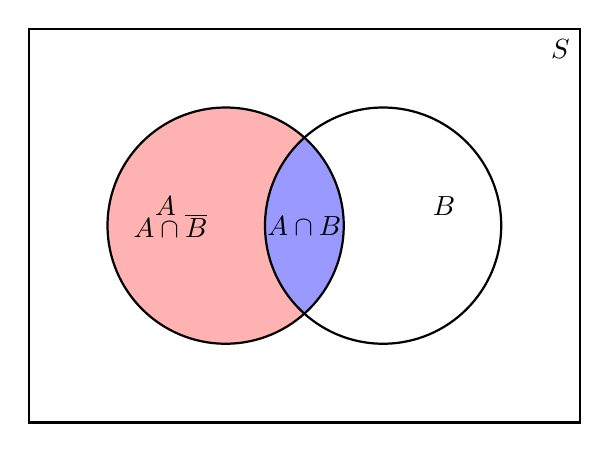
\begin{tikzpicture}[thick, set/.style={circle, minimum size=3cm}]
    % Universal Set
    \draw (-3,-2.5) rectangle (4,2.5) node[below left] {$S$};
    
    % Draw and Fill Sets
    % Fill A intersect not B
    \fill[red!30] (-0.5,0) circle (1.5cm);
    \fill[white] (1.5,0) circle (1.5cm);
    
    % Fill A intersect B
    \begin{scope}
        \clip (-0.5,0) circle (1.5cm);
        \fill[blue!40] (1.5,0) circle (1.5cm);
    \end{scope}

    % Draw borders
    \draw (-0.5,0) circle (1.5cm) node[above left, xshift=-0.5cm] {$A$};
    \draw (1.5,0) circle (1.5cm) node[above right, xshift=0.5cm] {$B$};

    % Labels
    \node at (-1.2, 0) {$A \cap \comp{B}$};
    \node at (0.5, 0) {$A \cap B$};
\end{tikzpicture}
\end{center}

\subsection{Heuristics \& "Cheats"}
\begin{itemize}
    \item \textbf{Permutation vs. Combination Hack:} If you can swap the assigned outcomes and it represents a *different* scenario in reality (e.g., Alice gets Job A, Bob gets Job B $\neq$ Alice gets Job B, Bob gets Job A), use Permutations ($P$). If swapping them yields the same physical state (e.g., Alice and Bob are both selected for the jury), use Combinations ($C$).
    \item \textbf{Complement Cheat:} Whenever a problem asks for ``at least one'' (as in 2.8), always calculate $1 - \Prob(\text{none})$. It shifts a difficult union of events into a single intersection.
\end{itemize}

\subsection{Pitfalls \& Fallacies}
\begin{itemize}
    \item \textbf{Conflating Mutually Exclusive with Independent:} Mutually exclusive sets ($A \cap B = \emptyset$) are \textit{highly dependent}. If $A$ happens, $B$ is guaranteed not to happen. Independence means $\Prob(A \cap B) = \Prob(A)\Prob(B)$. Never assume one implies the other.
    \item \textbf{Phantom Distinctness Fallacy:} Treating identical items as distinct when mapping the sample space cardinality. If you have 3 red balls, labeling them $R_1, R_2, R_3$ expands the sample space, which is fine \textit{only if} you apply the same distinctness metric to both your numerator (favorable) and denominator (total) probabilities.
\end{itemize}

\newpage
% ======================================================================= %
\section{Part 5: Conceptual Synthesis and The "Big Picture"}
% ======================================================================= %

\subsection{A) Thematic Connections}
The unified theme of this chapter is \textbf{Formalizing Randomness via Measure Theory}. By translating intuitive concepts of "chance" into strict set-theoretic axioms (unions, intersections, subsets), we strip away human bias. Combinatorics provides the computational engine (the cardinality metric $|E|$), while Kolmogorov’s axioms provide the chassis (the $\sigma$-algebra $\mathscr{F}$). 

\subsection{B) Forward and Backward Links}
Backwardly, this material relies on fundamental Boolean logic and set mappings introduced in early discrete mathematics. Forwardly, it serves as the absolute bedrock for:
\begin{itemize}
    \item \textbf{Random Variables \& Expected Value:} We will soon map the sample space $\Omega$ to the Real numbers using functions $X: \Omega \to \mathbb{R}$. Without a solid $\sigma$-algebra, ensuring these functions are mathematically measurable is impossible.
    \item \textbf{Lebesgue Integration:} In advanced probability theory, discrete summation $\sum \Prob(x_{i})$ transforms into the abstract Lebesgue integral $\int X d\mathbb{P}$, an absolute necessity for continuous distributions.
\end{itemize}


% ======================================================================= %
\section{Part 6: Abstract Real-World Modeling (AI, ML, \& Quant Finance)}
% ======================================================================= %

While rolling dice and dispatching taxis are trivial, the exact same mathematical structures power modern high-level engineering and finance.
\begin{itemize}
    \item \textbf{Generative AI (Diffusion Models):} The sample space $\Omega$ is an uncountably infinite dimension of pixel manifolds $\mathbb{R}^{d}$. Calculating the probability of a coherent image requires integrating over continuous measure spaces utilizing the exact principles of intersections (e.g., $\text{Image} \cap \text{Text Prompt Constraints}$).
    \item \textbf{Algorithmic Trading (Order Book State Spaces):} The sample points are discrete movements of an asset's price in a limit order book.
\end{itemize}

\subsection{Model Problem Setup: Quantitative Finance \& Option Pricing}
Consider modeling the probabilistic behavior of an underlying asset $S_{t}$ for pricing a European Call Option in a discrete binomial framework before advancing to continuous Stochastic Differential Equations.
\begin{definition}[Filtration and Probability Space]
Let $(\Omega, \mathscr{F}, \mathbb{P})$ be a probability space. The state space $\Omega = \{U, D\}^{T}$ represents a sequence of $T$ discrete time steps where the stock can move Up ($U$) or Down ($D$). We define a filtration $\mathbb{F} = \{\mathscr{F}_{t}\}_{t=0}^{T}$ which represents the accumulation of knowledge (the history of stock movements) up to time $t$. $\mathscr{F}_{t}$ is a $\sigma$-algebra where $\mathscr{F}_{0} = \{\emptyset, \Omega\}$ and $\mathscr{F}_{T}$ contains all individual sample paths.
\end{definition}

If a quantitative analyst models 3 time steps ($T=3$), there are $2^{3} = 8$ sample paths (exactly like the combinatorial spaces defined in Problem 2.19). A derivative contract pays off based on the terminal value $S_{T}$. Using the law of total probability, the Expected Value (price) under the risk-neutral measure $\mathbb{Q}$ is:
\[ C_0 = e^{-rT} \sum_{\omega \in \Omega} \max(S_T(\omega) - K, 0) \cdot \mathbb{Q}(\{\omega\}) \]
This establishes that combinations, set spaces, and probability measures are the absolute foundation of billion-dollar algorithmic derivatives pricing.

\newpage
% ======================================================================= %
\section{Part 7: Common Variations and Untested Concepts}
% ======================================================================= %

A critical theorem frequently tested in advanced probability courses but missing from the basic assignments provided is the generalized \textbf{Inclusion-Exclusion Principle for 3 Sets}. The problems tested $P(A \cup B)$, but real-world data overlaps multiple attributes.

\begin{theorem}[Inclusion-Exclusion for Three Sets]
For any three events $A, B, C \in \mathscr{F}$:
\[ \Prob(A \cup B \cup C) = \Prob(A) + \Prob(B) + \Prob(C) - \Prob(A \cap B) - \Prob(A \cap C) - \Prob(B \cap C) + \Prob(A \cap B \cap C) \]
\end{theorem}

\begin{proof}
Let $D = A \cup B$. We apply the two-set axiom:
\[ \Prob(A \cup B \cup C) = \Prob(D \cup C) = \Prob(D) + \Prob(C) - \Prob(D \cap C) \]
Substitute $D$ back in:
\[ \Prob(A \cup B \cup C) = \Prob(A \cup B) + \Prob(C) - \Prob((A \cup B) \cap C) \]
Expand $\Prob(A \cup B)$ and apply the distributive law to the intersection:
\[ \Prob(A \cup B \cup C) = \big[ \Prob(A) + \Prob(B) - \Prob(A \cap B) \big] + \Prob(C) - \Prob((A \cap C) \cup (B \cap C)) \]
Apply the two-set axiom again to the last term:
\[ \Prob((A \cap C) \cup (B \cap C)) = \Prob(A \cap C) + \Prob(B \cap C) - \Prob((A \cap C) \cap (B \cap C)) \]
Note that $(A \cap C) \cap (B \cap C) = A \cap B \cap C$. Substituting this back into the main equation yields:
\[ \Prob(A \cup B \cup C) = \Prob(A) + \Prob(B) + \Prob(C) - \Prob(A \cap B) - \Prob(A \cap C) - \Prob(B \cap C) + \Prob(A \cap B \cap C) \]
\end{proof}


% ======================================================================= %
\section{Part 8: Advanced Diagnostic Testing: "Find the Flaw"}
% ======================================================================= %

Below are 5 advanced proofs or solutions that appear perfectly logical but contain a subtle, critical mathematical flaw. Your task as a grader is to identify the flaw. \textit{Answers are provided in the key at the bottom.}

\textbf{Flawed Problem 1: Mutually Exclusive Properties}
\textit{Proof statement:} Let $A$ and $B$ be two non-empty events. If $\Prob(A) = 0.6$ and $\Prob(B) = 0.5$, then $A$ and $B$ can be mutually exclusive events.
\textit{Flawed Proof:} By definition, mutually exclusive events have an intersection of zero, $\Prob(A \cap B) = 0$. The probability of their union is $\Prob(A \cup B) = \Prob(A) + \Prob(B) = 0.6 + 0.5 = 1.1$. This is just a theoretical sum, establishing the spaces are distinct. $\blacksquare$

\textbf{Flawed Problem 2: The Poker Double-Count}
\textit{Question:} Find the probability of drawing exactly one pair (e.g., two 8s, and three other cards of distinct ranks) in a 5-card poker hand.
\textit{Flawed Solution:} Total hands is $\binom{52}{5}$. First, choose the rank for the pair: $\binom{13}{1}$. Choose 2 suits for the pair: $\binom{4}{2}$. Then choose 3 other cards from the remaining 48 cards to complete the 5-card hand: $\binom{48}{3}$. The probability is $\frac{\binom{13}{1}\binom{4}{2}\binom{48}{3}}{\binom{52}{5}}$. $\blacksquare$

\textbf{Flawed Problem 3: Uniform Infinite Measures}
\textit{Question:} Let the sample space be all natural numbers $\Omega = \mathbb{N}$. Prove that we can define a uniform probability distribution over $\mathbb{N}$ where every integer is equally likely to be selected.
\textit{Flawed Proof:} Let $\Prob(n) = c$ for all $n \in \mathbb{N}$. Since the space is infinite, as $N \to \infty$, $c = \lim_{N \to \infty} \frac{1}{N} = 0$. Since $\Prob(n) \ge 0$, this satisfies Kolmogorov's first axiom. Therefore, the uniform measure is valid. $\blacksquare$

\textbf{Flawed Problem 4: Set Subset Algebra}
\textit{Proof statement:} If $A \cup B = A \cup C$, then $B = C$.
\textit{Flawed Proof:} Assume $A \cup B = A \cup C$. Intersect both sides of the equation with the complement of $A$ ($\comp{A}$):
$(A \cup B) \cap \comp{A} = (A \cup C) \cap \comp{A}$.
By distribution: $(A \cap \comp{A}) \cup (B \cap \comp{A}) = (A \cap \comp{A}) \cup (C \cap \comp{A})$.
This simplifies to $\emptyset \cup (B \cap \comp{A}) = \emptyset \cup (C \cap \comp{A})$, which implies $B \cap \comp{A} = C \cap \comp{A}$. Therefore, $B = C$. $\blacksquare$

\textbf{Flawed Problem 5: Conditional Divisors}
\textit{Proof statement:} For any three events $A, B, C$, $\Prob(A \mid B \cap C) = \frac{\Prob(A \cap B \mid C)}{\Prob(B \mid C)}$.
\textit{Flawed Proof:} 
Using the definition of conditional probability:
$\frac{\Prob(A \cap B \mid C)}{\Prob(B \mid C)} = \frac{\frac{\Prob(A \cap B \cap C)}{\Prob(C)}}{\frac{\Prob(B \cap C)}{\Prob(C)}}$.
The $\Prob(C)$ cancels out, leaving $\frac{\Prob(A \cap B \cap C)}{\Prob(B \cap C)}$, which by definition is $\Prob(A \mid B \cap C)$. $\blacksquare$

\vspace{0.5cm}
\hrule
\vspace{0.5cm}

\subsubsection*{Diagnostic Solution Key}
\begin{enumerate}
    \item \textbf{Flaw 1:} The flaw lies in the result $\Prob(A \cup B) = 1.1$. This violates Kolmogorov's Second Axiom, which mandates that for any event $E \in \mathscr{F}$, $\Prob(E) \le 1$. Therefore, they \textit{cannot} be mutually exclusive; they must have an overlap of at least 0.1.
    \item \textbf{Flaw 2:} Combinatorial double-counting. By selecting any 3 cards from the remaining 48 via $\binom{48}{3}$, the subset might contain a \textit{second} pair, or a three-of-a-kind, violating the ``exactly one pair'' condition. The correct logic requires choosing 3 distinct ranks from the remaining 12 ranks: $\binom{12}{3} \times \binom{4}{1}^3$.
    \item \textbf{Flaw 3:} The flaw is violating Kolmogorov's Third Axiom (Countable Additivity). If $c = 0$, then $\sum_{n \in \mathbb{N}} \Prob(n) = \sum_{n \in \mathbb{N}} 0 = 0$. But $\Prob(\Omega)$ must equal 1. Thus, a uniform probability measure over a countably infinite set cannot exist.
    \item \textbf{Flaw 4:} The logic proves that $B \cap \comp{A} = C \cap \comp{A}$, meaning the parts of $B$ and $C$ \textit{outside} of $A$ are equal. It completely fails to account for the components of $B$ and $C$ that reside \textit{inside} $A$. For example, if $B = \{1\}$ and $C = \{1, 2\}$, and $A = \{1, 2\}$, $A \cup B = A \cup C$ holds true, but $B \neq C$.
    \item \textbf{Flaw 5:} The algebraic cancellation looks flawless, but it contains a critical, hidden assumption: It fails to stipulate that $\Prob(B \cap C) > 0$. If $\Prob(B \cap C) = 0$, the denominator $\Prob(B \mid C) = 0$, leading to division by zero. Conditional probability is undefined for conditioning on a zero-probability measure event.
\end{enumerate}

\end{document}